\chapter{INTRODUCTION} \label{chapter:introduction}

\noindent \textit{How many Gr\'evy's zebra are in Kenya?}

\hfill

\noindent The Gr\'evy's zebra (\textit{Equus grevyi}), as seen in Figure~\ref{fig:grevys}, was last assessed in 2016 as \textit{Endangered} by the IUCN Red List\footnote{IUCN Red List for Gr\'evy's Zebra: \url{https://www.iucnredlist.org/species/7950/89624491} (Accessed: Oct. 29, 2021).}.  This crucial designation marks the estimated probability of extinction for this species at 20\% (or above) over the next five generations.  The population in the late 1980s was estimated to be around 5,800 animals, whereas the population today is believed to be about half that number~\cite{rubenstein_equus_2016}.  As with all species, the apparent health of the Gr\'evy's zebra population is linked to its total number of members. Agonizingly, however, their population numbers have not been tracked closely or consistently within Kenya, their primary country of residence.  This lack of clarity presents a literal existential challenge for conservationists, where having access to a reliable, species-level population estimate is foundational to evaluating the impact of conservation policy and monitoring the growth or decline of the species.\blfootnote{Portions of this chapter previously appeared as: J. Parham and C. Stewart, ``Detecting plains and Grevy’s zebras in the real world,'' in \textit{IEEE Winter Conf. Applicat. Comput. Vis. Workshops}, Lake Placid, NY, USA, Mar. 2016, pp. 1–9.}\blfootnote{Portions of this chapter previously appeared as: J. Parham, J. Crall, C. Stewart, T. Berger-Wolf, and D. I. Rubenstein, ``Animal population censusing at scale with citizen science and photographic identification,'' in \textit{AAAI Spring Symp.}, Palo Alto, CA, USA, Jan. 2017, pp. 37–44.}

\begin{figure}[!t]
    \begin{center}
        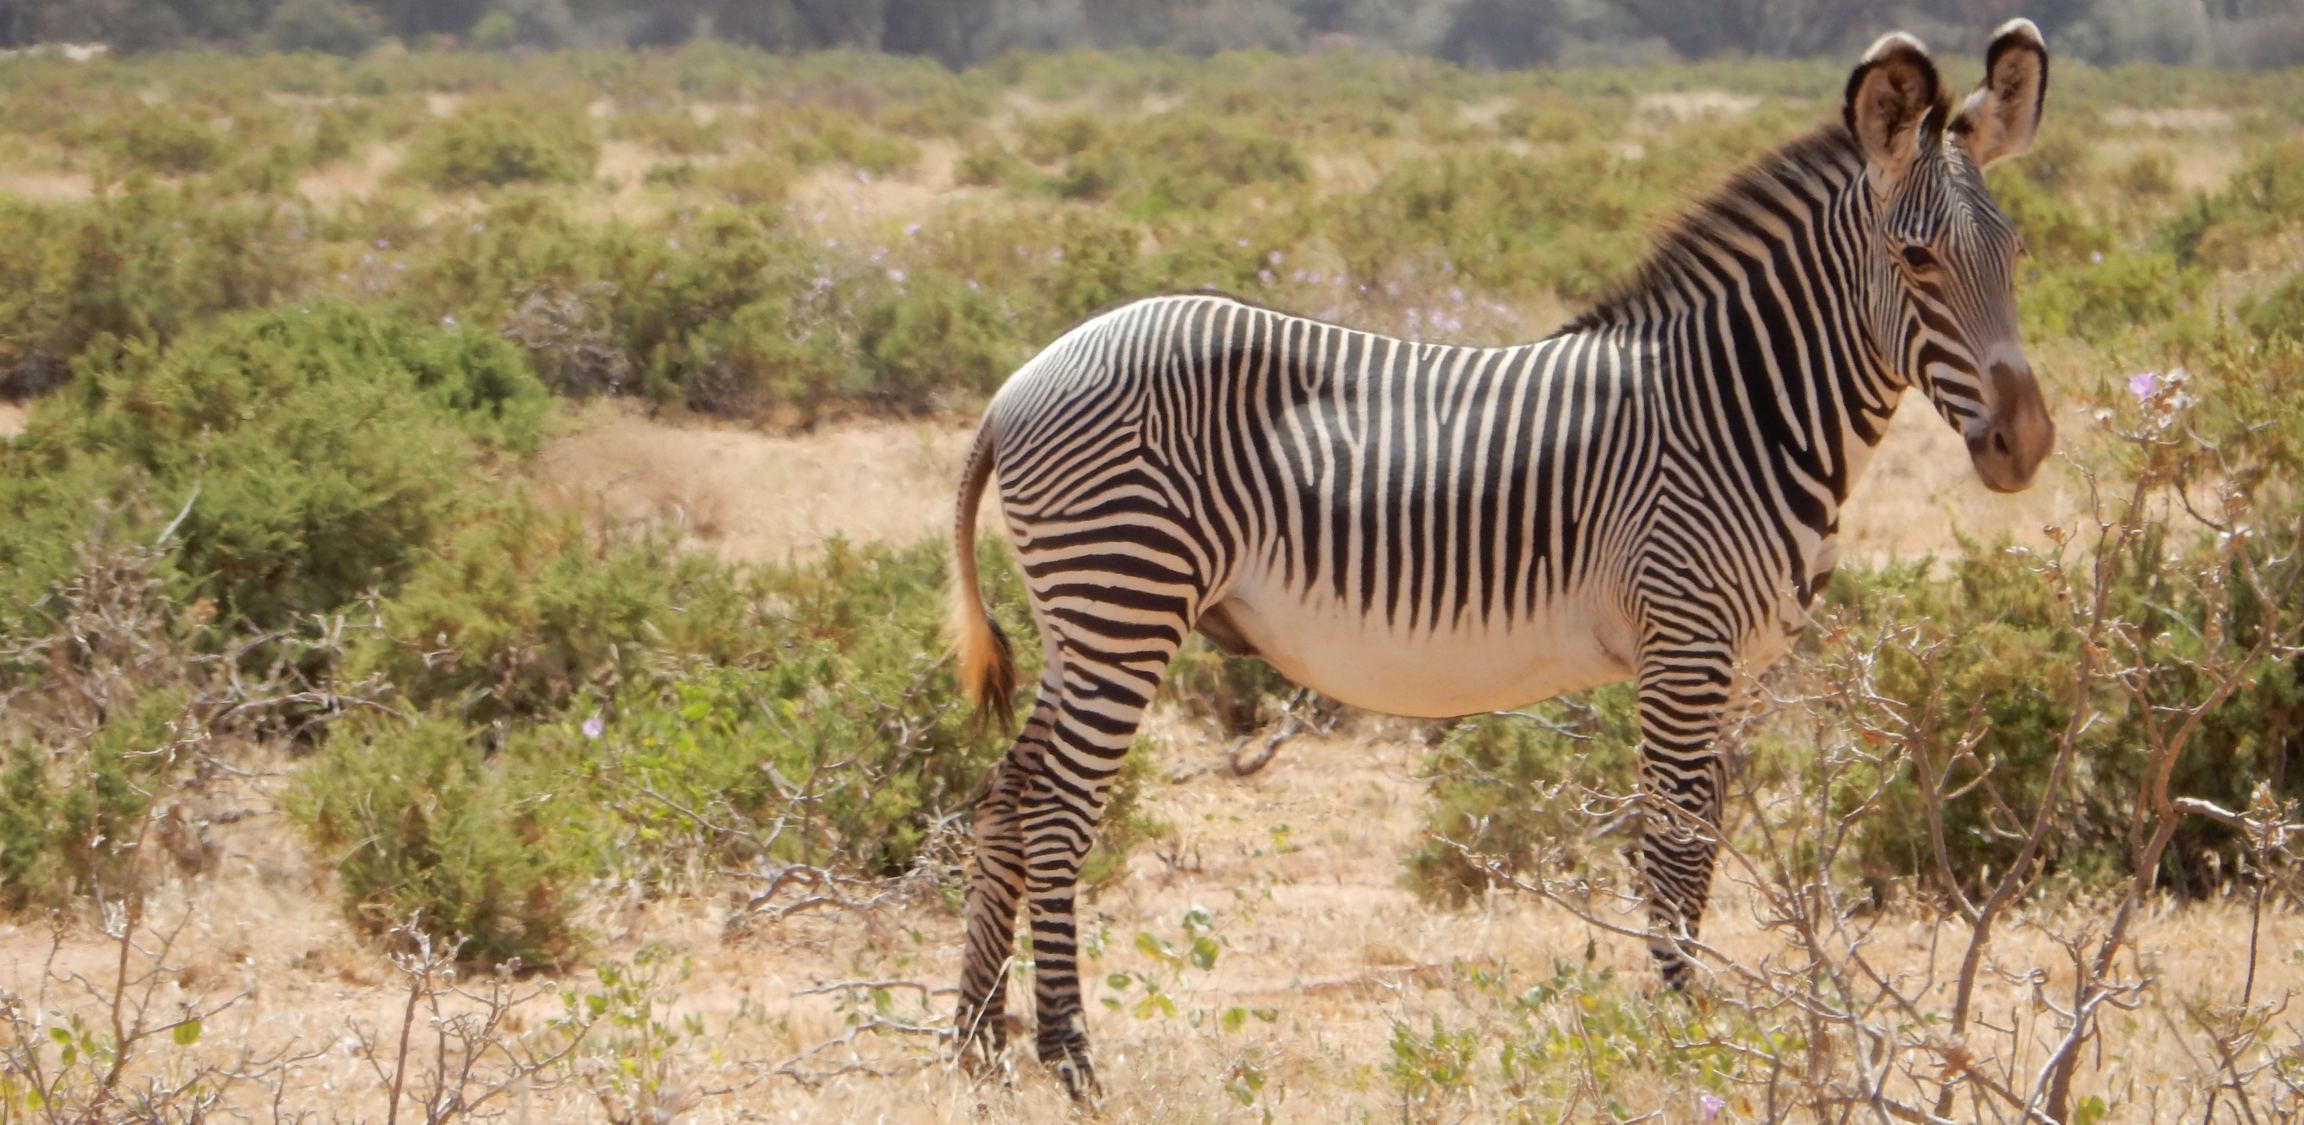
\includegraphics[width=0.8\linewidth]{resources/grevys-color.pdf}
    \end{center}
    \caption{An image of a Gr\'evy's zebra in Kenya.  Grevy's zebra have thin stripes across the body and a white underbelly.  Approximately 90\% of the world's Gr\'evy's zebra are located in Kenya~\cite{rubenstein_equus_2016}.}
    \label{fig:grevys}
\end{figure}

To better track its overall health, we would ideally like to perform a \textit{census} of the entire species and be able to do it routinely.  A census is distinct from a simple count as the former tracks \textit{individual} animals over time\footnote{This discussion borrows language commonly used for people; for simplicity, it refers to animals as ``individuals''.}.  For example, a census allows researchers to estimate the population size, but it also gathers data that can be used to answer important ecological questions like, ``\textit{where are the animals migrating to and from?}'', ``\textit{what areas are isolated by geography or human development?}'', ``\textit{who are the members of an animal's social group, and do those groups change?}''\ or a question as basic as ``\textit{what is the average life expectancy in the wild?}''  These questions are hard to answer if we only count and record the number of animals seen at a given place and time~\cite{fitzgibbon_antipredator_1995,ginsberg_social_1988,tombak_behavioral_2019,keesing_impacts_1998,kivai_feeding_2006,rubenstein_ecology_1994,zero_monitoring_2013}.  Anonymity is what limits the usefulness of animal population monitoring.  A regular census of known individuals allows for a more intimate and up-to-date understanding of the animal population, which is critical when a species is threatened.

Biologists have long used physical tagging to track individuals and estimate animal population sizes.  One of the most popular and prevalent techniques for producing a population size estimate is capture-mark-recapture~\cite{robson_sample_1964,pradel_utilization_1996} (or simply ``mark-recapture'').  Mark-recapture is a sampling technique that starts with an initial capture of the animal population.  A second independent capture of the same population is then performed. The number of recaptured animals between the first and second collections is used to estimate the number of animals that were not captured at all.  An ecologist may choose to mark the animals from the first capture with paint or use some other type of physical tag to know which animals have been seen before.  Performing this kind of detailed mark-recapture study can be prohibitively demanding when the number of individuals in a population grows too large, the population moves across too large of a distance, or the species is difficult to capture due to evasiveness or habitat inaccessibility~\cite{seber_estimation_1982}.  Moreover, marking with physical tagging methods like ear tags, metal bands, ear notches, skin branding, or GPS collars can be unreasonably invasive, laborious, expensive, or alter the animal's behavior.  These challenges limit how often mark-recapture studies are performed and how comprehensively they can sample the population.

\begin{table}[!t]
    \caption{A comparison of photographic censusing to existing population estimation methodologies demonstrates that it is better for large animal populations.}
    \label{table:comparison}
    \begin{center}
        \begin{tabular}{| c | c |}
            \hline
            \textbf{Traditional Methods}                          & \textbf{Photographic Censusing}                        \\
            \hline
            \textbf{invasive}                                     & \textbf{passive}                                       \\
            ear notches, tags, radio collars                      & appearance-based with computer vision,                 \\
            tranquilizers and veterinary services                 & does not influence behavior of animals                 \\
            \hline
            \textbf{expensive}                                    & \textbf{inexpensive}                                   \\
            logistically demanding on research                    & distributed, can utilize volunteers                    \\
            staff and park rangers, requires                      & and tourists, specialized equipment                    \\
            specialized equipment and training                    & and training not required                              \\
            \hline
            \textbf{error-prone}                                  & \textbf{evidence-based}                                \\
            double counting, human                                & machine learning and computer vision,                  \\
            interpretation of data required,                      & data-driven decisions, human-in-                       \\
            tedious verification                                  & the-loop verification, statistical estimate            \\
            \hline
            \textbf{one-time analysis}                            & \textbf{recurring}                                     \\
            difficult to repeat over time,                        & allows for tracking individuals over                   \\
            based on verbal reports                               & time, ecological trends are available,                 \\
            cannot audit later                                    & audit with newer algorithms                            \\
            \hline
            \textbf{\color{red} Infeasible for large populations} & \textbf{\color{darkgreen} Ideal for large populations} \\
            \hline
        \end{tabular}
    \end{center}
\end{table}

Instead, we would prefer to leverage an animal's intrinsic appearance to ``mark'' if it has been seen before, taking advantage of a faster and more passive capture process: sight.  A better version of mark-recapture can be created that is based on \textit{sights} and \textit{resights} of animals while still relying on the same underlying methodology for estimating the population size.  Suppose the visual appearances are unique for each animal in a population and that humans can distinguish two animals based only on their natural markings. In that case, a sight-resight study can be used to track encounters of new and known individuals.  In short, if we apply this idea to Gr\'evy's zebras, we can think of them almost as walking fingerprints.  Just like human thumbprints are unique and linked to a person's identity, the stripe patterns on the side of a zebra are distinctive and unique to that individual.  While it is clear that appearance-based ID will not work universally for all species (e.g., a brown squirrel or the skin of a sleek, grey dolphin), we can expect that a giraffe's unique blanket of brown patches, or the intricate layout of scutes on a sea turtle's flipper, or the jagged outline of a whale fluke can be used to recognize and distinguish unique animals.

Expecting a person to remember and recognize hundreds -- let alone thousands -- of individuals by sight is unrealistic. Therefore, some method of cataloging is needed to help keep records of the animals that have been seen.  As the catalog grows, however, the amount of work required to keep tabs on an ever-increasing number of animals can become too demanding or error-prone.  Doing this work by hand with notes or physical pictures is therefore not a scalable solution.  One straightforward option is to use computational aides that can help store, sort, retrieve, compare, and curate a digital catalog (i.e., a database) of the different encountered animals.  Digital photographs are ideal when building such an appearance-based digital catalog of animal IDs as they are easy to capture and store.  Furthermore, taking a photograph of an animal allows for the passive collection of its identifying information and provides a piece of evidence for who, when, and where that individual was seen.  A digital image is convenient not only because humans or algorithms can review it to build the database, but it can also be retrieved and re-examined in the future.  An audit cannot be done with hand-written accounts for the number of animals in an area.

The transition towards using computers and digital photography, by itself, does not change the underlying amount of work that is needed to manage the catalog. However, as alluded to earlier, automation is needed to make the workload manageable.  A primary benefit of using digitized photographic data is that computer vision algorithms can automate laborious tasks.  This dissertation introduces the novel concept of \textit{photographic censusing}, a comprehensive and bootstrapable process that uses 1) digital images of animals as input, 2) computer vision algorithms to automate the vast majority of the work needed from humans, and 3) a database to record unique individuals and their respective sightings.  Photographic censusing is designed to be scalable; a large geographic area can be surveyed by adding additional, independent photographers, and the method has been experimentally validated \textit{in situ} for large animal populations with thousands of members.  Table~\ref{table:comparison} provides a summary of photographic censusing and a comparison to existing methods.

\section{Animal Detection}

Two high-level computer vision components, detection and identification (ID), are required to perform an automated census of animals from photographs.  Most of the attention is paid to state-of-the-art identification algorithms in animal censusing, but the role of detection is vital as a required pre-condition for ID, and it is considered carefully here.  The detection component analyzes the original photographs and produces a collection of smaller, more focused cropped regions -- called \textit{annotations} -- around the animals that are of interest for the census.  The identification process then takes the annotations and groups them into a database of unique individuals.  The detection component must be able to do the following tasks automatically:

\begin{enumerate}
    \item locate an indeterminate number of animals in a photograph,
    \item determine if the animal is relevant to the census (e.g., the desired species),
    \item remove visual information that may distract or otherwise confuse identification, and
    \item filter out animals that are ultimately not identifiable (not useful in a census).
\end{enumerate}

\begin{figure}[!t]
    \begin{center}
        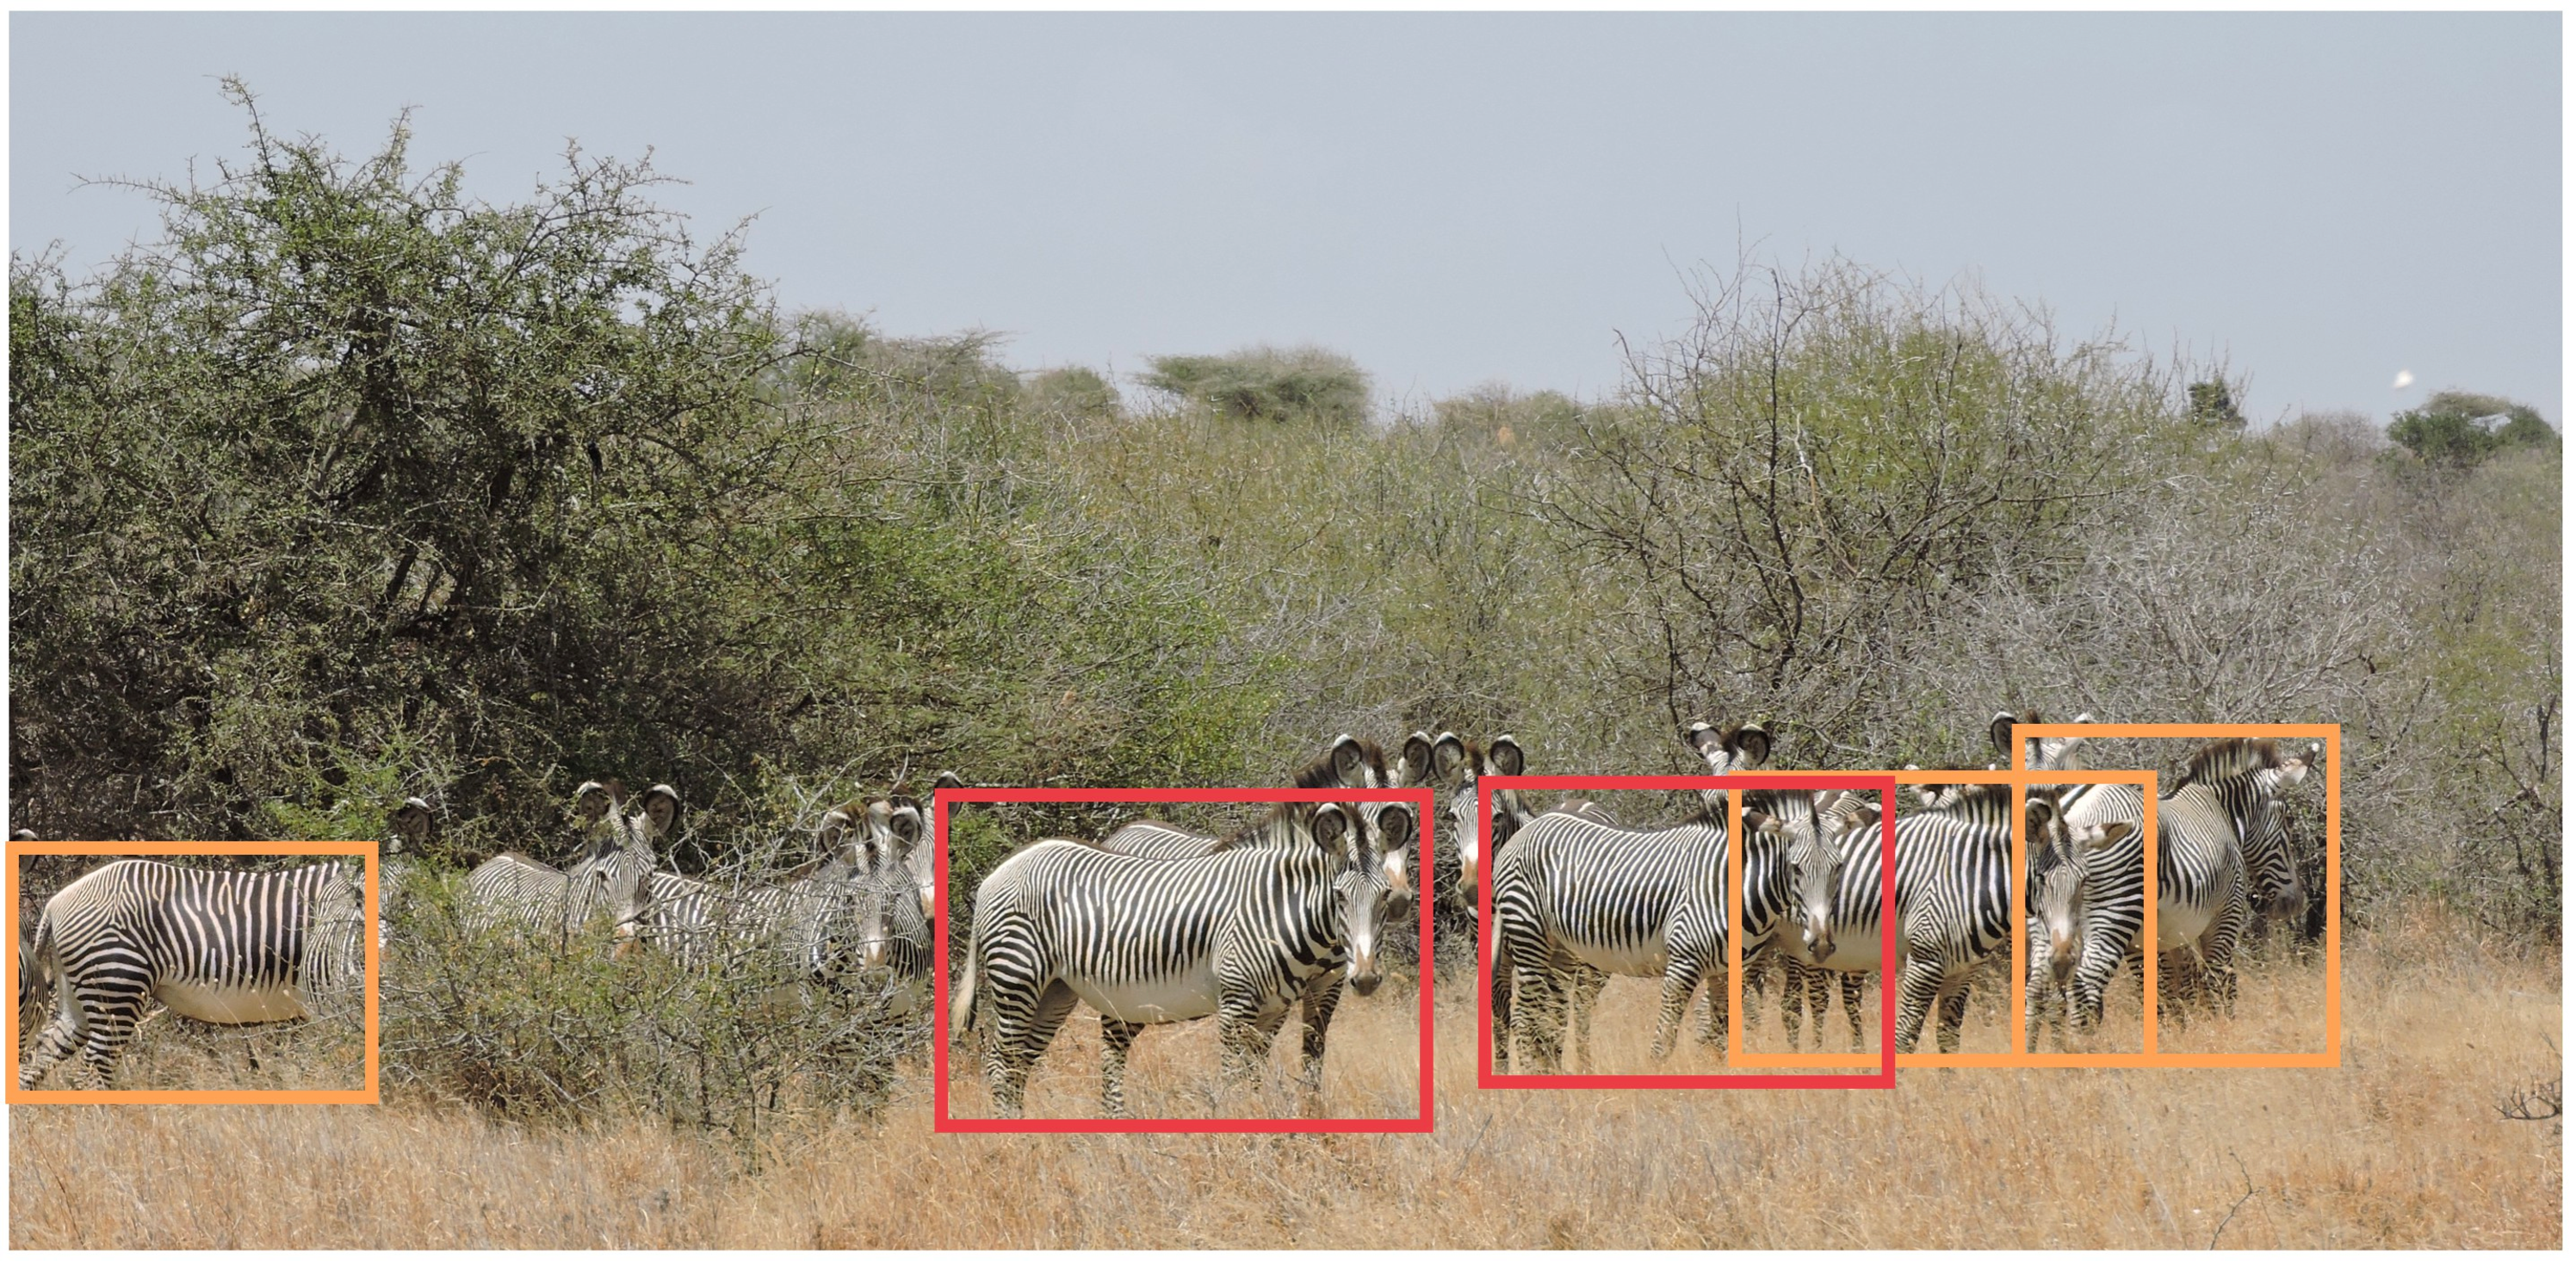
\includegraphics[width=1.0\linewidth]{resources/clutter-annotated.pdf}
    \end{center}
    \caption{An image of a herd of Gr\'evy's zebra in Kenya.  The computer vision task of detection is very challenging when considering overlapping animals, each with a different pose and level of occlusion.  The red boxes are identifiable animals whereas the orange boxes have a hip or shoulder region obscured (both of which are required for reliable and automated ID).  All other animals are too occluded or truncated to be identified.}
    \label{fig:clutter}
\end{figure}

\noindent To achieve these requirements, we need to expand the classic definition of object detection in computer vision.  Object detection typically refers to the task of placing bounding boxes around \textit{all} objects of interest in a photograph.  This formulation places too much importance on completeness.  For example, consider Figure~\ref{fig:clutter} which shows a dense herd of 15 Gr\'evy's zebras\footnote{The reader is encouraged to try and count the number of animals, including the sliver of an animal on the far left.}.  What is to be considered the ``correct'' output of an object detection algorithm for this image?  The traditional answer would be to produce a complete set of bounding boxes for each of the 15 animals regardless of their size and clarity.  However, this would be inappropriate for use in a census because not all animals are identifiable.  For example, the obscured animals behind the bush on the left side of the frame are not seen clearly and should not be provided to an appearance-based identification process.

A more suitable definition of object detection would be aware that some annotations are not worth trying to find, recognizing that it is safe to ignore animals that are ultimately not going to be identifiable. For example, in Figure~\ref{fig:clutter} the two most foreground animals (bordered in red) are reliably identifiable, with three additional annotations (orange) that may be identifiable in some cases.  All other animals and detections in this image should be considered distractions. A detection process optimized for use in a photographic census should only produce the 2-5 highlighted boxes as output.  The detection process also needs to recognize the species, and even the viewpoint, of interest for a census.  Just as people's left and right thumbprints are different, the visual appearances on an animal's left and right sides are different.  It would be imprudent for an identification process to compare one person's left thumbprint against another person's right thumbprint because they are fundamentally incomparable. Likewise, how could you tell if a right viewpoint zebra and a left viewpoint zebra were the same animal?  Without being able to view the same areas on the bodies and compare corresponding stripe patterns, you would likely be unable to decide \textit{yes} or \textit{no}.  The detector needs to go beyond simply creating annotations and should actively try to prevent incomparable matches.  The detection process is expected to provide a semantic understanding of the annotations given to ID and filter them appropriately to reduce errors and prevent the need for a human to intervene.

\begin{figure}[!t]
    \begin{center}
        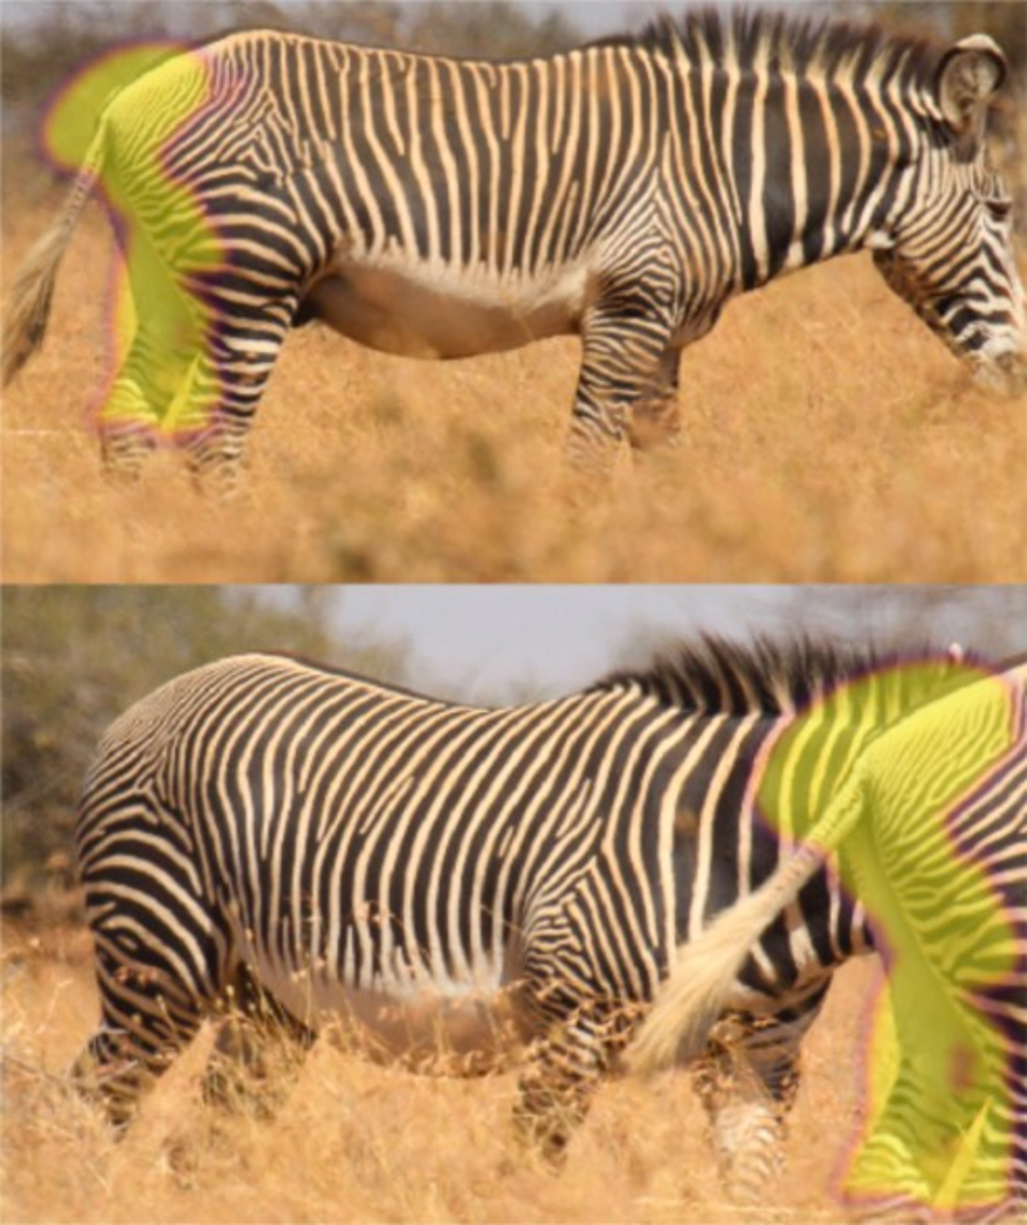
\includegraphics[width=0.6\linewidth]{resources/photobomb.pdf}
    \end{center}
    \caption{An example of a Gr\'evy's zebra photobomb.  A photobomb occurs when the same animal is matched between two annotations but the \textit{primary} animal in both annotations is different.}
    \label{fig:photobomb-overview}
\end{figure}

An appearance-based identification process can also be fairly sensitive to poorly-formed annotations. One example is a ``photobomb'', as seen in Figure~\ref{fig:photobomb-overview}.  A visual matching algorithm called HotSpotter~\cite{crall_identifying_2017} (discussed later in this dissertation) was used to search a database of annotations for likely matches, and this pair was returned with a high score.  It is clear that the identification process is correctly matching the appearance of the same animal between these two annotations, but not between the \textit{intended} (or primary) animals those annotations are meant to represent.  The error that identification has made is understandable -- and from its perspective of finding visual correspondences between two annotations is perfectly valid -- but ultimately incorrect.  The error is possible because the ID algorithm lacks a deeper semantic understanding of which areas (and animals) are being matched.  In contrast, we can also frame this example as a failure of detection to properly limit the visual appearance to only the most relevant and comparable regions.  If the bottom image were cropped to exclude the animal to the right and focus on the body region, this visual match would not have been made.  Reducing these types of ``incidental matches'' improves the overall automation of the identification process because when failures like this happen, it is often left to a human reviewer to find and fix the issue.

In summary, animal detection is tasked with providing a semantic but filtered understanding of the world to ID.  There is a trade-off between producing relevant, identifiable, and comparable annotations and the amount of work needed to find and fix mistakes poor annotations cause during identification.  Accordingly, filtering out irrelevant, unidentifiable, or incomparable annotations is similar to pretending the sighting of that animal never happened in the first place.  Since photographic censusing, as a sight-resight study, is based on sampling, it does not expect every animal in the population to be photographed.  We can thus rely on filtering to control the completeness of the analysis and balance it against the amount of work humans need to do to produce the population estimate.

\section{Contributions}

This dissertation presents an end-to-end process for animal population monitoring at scale.  High degrees of automation, and bootstrapable machine learning components, allow photographic censusing to be performed quickly and accurately, enabling a new and realistic option for data-driven animal conservation.  This dissertation offers the following contributions:

\begin{enumerate}
    \item \textbf{Animal Detection Pipeline} - a comprehensive detection pipeline for animals for use in photographic censusing.  The pipeline is designed to be easily bootstrapable for new species with relatively minimal amounts of ground truth annotations.  The pipeline is constructed out of modularized components, including a whole-image classifier, an annotation and part bounding box localizer, a bounding box orientation regression network, an annotation species and viewpoint labeler, an annotation-part assigner, a coarse background segmentation network, and an Annotation of Interest (AoI) classifier.  The pipeline is not limited to Gr\'evy's zebra or herding species and can even be used with multiple species of interest in the same image, on overhead imagery, and with camera trap data.  The discussion throughout will use Gr\'evy's zebra as a motivating example due to the availability of large-scale and novel ground-truth detection and ID datasets.
    \item \textbf{Animal Datasets} - five new public datasets for animal detection and ID research.  Common public datasets for computer vision tasks like object detection generally do not provide associated ID information when they include boxes of animals.  Likewise, animal ID datasets often only include pre-cropped images of animals and rarely focus on herding species.  The largest contributed dataset focuses on Gr\'evy's zebra IDs and is highly curated.  The dataset aggregates 5,464 real-world images taken from two large censusing rallies, includes hand-drawn and labeled annotations for Gr\'evy's zebra and 22 other species, and provides ground-truth ID labels for 554 unique animals.  Two detection datasets are also made available that have ground-truth bounding boxes and other metadata for multiple species.  Lastly, the GGR-16 and GGR-18 datasets will also be made available for ecological research.
    \item \textbf{Census Annotation} - a novel concept that is designed to reduce incomparable and incidental matching during animal identification.  The concept is implemented with two components: 1) a Census Annotation (CA) classifier and 2) a Census Annotation Region (CA-R) regression network.  The CA classifier filters out unidentifiable annotations and allows ID only to see the most identifiable annotations during a photographic census.  The CA-R network creates more focused regions within existing detected annotations, drastically reducing the amount of human effort by increasing the separability of automated ID verifiers.
    \item \textbf{Photographic Censusing Rallies} - an organized data collection event where ``citizen scientist'' volunteer photographers are trained and tasked to take photos of animals for two back-to-back days.  The results of the Great Gr\'evy's Rally 2016 (GGR-16) and Great Gr\'evy's Rally 2018 (GGR-18) censusing rallies are significant contributions of this work.  Those two rallies are a refinement and extension of the proposed methodology used during the Great Zebra \& Giraffe Count (GZGC), the focus of the author's master's thesis~\cite{parham_photographic_2015}.  The GGR-16 and GGR-18 rally procedures were significantly improved by increasing the automation of the detection and identification processing, streamlining data collection with GPS-enabled cameras, and proving that the original methodology scales to thousands of animals. In addition, the GGR events collected nearly an order of magnitude more images with twice as many contributors than the GZGC.  As a result, they offer the ideal database and framework for analyzing the impact of the automated detection pipeline and CA on real-world data.
\end{enumerate}

Lastly, here is a brief overview of the impact of the methods introduced in this work.  The original processing of the GGR-16 and GGR-18 census results was completed with large amounts of human effort.  The analysis of GGR-18 utilized 10,044 hand-picked annotations, formed a database of 1,972 unique individuals, and estimated that the population of Gr\'evy's zebra in Kenya was 2,812$\pm$171 animals (CI 95\%).  The processing was done with relatively experimental algorithms at the time and took approximately three months to complete.  It involved dozens of volunteers in drawing and labeling annotation bounding boxes, required 18,556 human decisions of annotation pairs suggested by an ID algorithm, and was estimated internally to cost at least \$50,000 USD in time and contracted labor.  Using the latest detection methods described in this dissertation, together with a new ID ranking algorithm, all of the original 56,588 images were re-processed.  Without any human effort, 11,916 annotations were found that showed identifiable, comparable, right-side Gr\'evy's zebra, with the detection processing taking approximately half a day to complete.  After approximately 12 more hours of completely automated ID ranking and automated pair review, a total of 1,297 human decisions were requested before the population estimate converged (it took one reviewer approximately 8 hours to complete). The new process estimated 2,820$\pm$167 Gr\'evy's zebra in Kenya in 2018, created a database of 2,022 unique animals (off by +2.5\% IDs compared to the GGR-18 database), and took approximately two working days to generate a result with one human reviewer.  If we assume that the reported GGR-18 census results were correct, then the new re-processed population estimate was accurate within 0.3\% and had a 93\% reduction in human effort.

The remaining chapters of this dissertation are organized as follows.  Chapter~\ref{chapter:related} provides a literature review of related work for deep learning in computer vision, supervised detection and classification methodologies, and existing population estimation techniques.  Chapter~\ref{chapter:detection} describes the detection pipeline, its machine learning components and introduces two new datasets for animal detection.  Chapter~\ref{chapter:overview} describes the process of photographic censusing, discusses what kinds of problems must be solved when automation is a primary goal during a census, and offers a mathematical framework for estimating a population size when machine learning methods are involved.  Chapter~\ref{chapter:overview} also introduces a new evaluation dataset for Gr\'evy's zebra ID that focuses on providing both ideal and compromised (i.e., hard) annotations.  Chapter~\ref{chapter:ca} introduces Census Annotations and Census Annotation Regions as a solution to the problem of incidental matching and other challenging scenarios that make human and automated processing more difficult.  Chapter~\ref{chapter:censusing} applies the concept of photographic censusing in the real world through photographic censusing rallies.  The Great Gr\'evy's Rally in 2016 (GGR-16) and the Great Gr\'evy's Rally in 2018 (GGR-18) were two large-scale photographic censusing events that generated population estimates for Gr\'evy's zebra and reticulated giraffe (\textit{Giraffa camelopardalis reticulata}) in Kenya, which are made available as two new ID datasets. Finally, Chapter~\ref{chapter:conclusion} provides a summary of the presented research, offers a discussion on its role within computer science, and suggests avenues for future work in automated wildlife conservation.
